%%%%%%%%%%%%%%%%%%%%%%%%%%%%%%%%%%%%%%%%%%%%%%%%
%% Intro to LaTeX and Template for Homework Assignments
%% Quantitative Methods in Political Science
%% University of Mannheim
%% Fall 2018
%%%%%%%%%%%%%%%%%%%%%%%%%%%%%%%%%%%%%%%%%%%%%%%%

% created by Marcel Neunhoeffer & Sebastian Sternberg


% This template and tutorial will help you to write up your homework. It will also help you to use Latex for other assignments than this course's homework.

%%%%%%%%%%%%%%%%%%%%%%%%%%%%%%%%%%%%%%%%%%%%%%%%
% Before we get started
%%%%%%%%%%%%%%%%%%%%%%%%%%%%%%%%%%%%%%%%%%%%%%%%

% Make an account on overleaf.com and get started. No need to install anything.

%%%%%%%%%%%%%%%%%%%%%%%%%%%%%%%%%%%%%%%%%%%%%%%%
% Or if you want it the nerdy way...
% INSTALL LATEX: Before we can get started you need to install LaTeX on your computer.
				% Windows: http://miktex.org/download
				% Mac:         http://www.tug.org/mactex/mactex-download.html	
				% There a many more different LaTeX editors out there for both operating systems. I use TeXworks because it looks the same on Windows and Mac.
				

% SAVE THE FILE: The first thing you need to do is to save your LaTeX file in a directory as a .tex file. You will not be able to do anything else unless your file is saved. I suggest to save the .tex file in the same folder with your .R script and where you will save your plots from R to. Let's call this file template_homework1.tex and save it in your Week 1 folder.


% COMPILE THE FILE: After setting up your file, using your LaTeX editor (texmaker, texshop), you can compile your document using PDFLaTeX.
	% Compiling your file tells LaTeX to take the code you have written and create a pdf file
	% After compiling your file, in your directory will appear four new files, including a .pdf file. This is your output document.
	% It is good to compile your file regularly so that you can see how your code is translating into your document.
	
	
% ERRORS: If you get an error message, something is wrong in your code. Fix errors before they pile up!
	% As with error messages in R, google the exact error message if you have a question!
%%%%%%%%%%%%%%%%%%%%%%%%%%%%%%%%%%%%%%%%%%%%%%%%


% Now again for everyone...

% COMMANDS: 
	% To do anything in LaTeX, you must use commands
	% Commands tell LaTeX when to start your document, how you want your document to look, and how to format your document
	% Commands ALWAYS begin with a backslash \

% Everything following the % sign is a comment and will not be used by Latex to compile your document.
% This is very similar to # comments in R.

% Every .tex file usually consists of four parts.
% 1. Document Class
% 2. Packages
% 3. Header
% 4. Your Document

%%%%%%%%%%%%%%%%%%%%%%%%%%%%%%%%%%%%%%%%%%%%%%%%
% 1. Document Class
%%%%%%%%%%%%%%%%%%%%%%%%%%%%%%%%%%%%%%%%%%%%%%%%
 
 % The first command you will always have will declare your document class. This tells LaTeX what type of document you are creating (article, presentation, poster, etc). 
% \documentclass is the command
% in {} you specify the type of document
% in [] you define additional parameters
 
\documentclass[a4paper,12pt]{article} % This defines the style of your paper

% We usually use the article type. The additional parameters are the format of the paper you want to print it on and the standard font size. For us this is a4paper and 12pt.

%%%%%%%%%%%%%%%%%%%%%%%%%%%%%%%%%%%%%%%%%%%%%%%%
% 2. Packages
%%%%%%%%%%%%%%%%%%%%%%%%%%%%%%%%%%%%%%%%%%%%%%%%

% Packages are libraries of commands that LaTeX can call when compiling the document. With the specialized commands you can customize the formatting of your document.
% If the packages we call are not installed yet, TeXworks will ask you to install the necessary packages while compiling.

% First, we usually want to set the margins of our document. For this we use the package geometry. We call the package with the \usepackage command. The package goes in the {}, the parameters again go into the [].
\usepackage[top = 2.5cm, bottom = 2.5cm, left = 2.5cm, right = 2.5cm]{geometry} 

% Unfortunately, LaTeX has a hard time interpreting German Umlaute. The following two lines and packages should help. If it doesn't work for you please let me know.
\usepackage[T1]{fontenc}
\usepackage[utf8]{inputenc}

% The following two packages - multirow and booktabs - are needed to create nice looking tables.
\usepackage{multirow} % Multirow is for tables with multiple rows within one cell.
\usepackage{booktabs} % For even nicer tables.

% As we usually want to include some plots (.pdf files) we need a package for that.
\usepackage{graphicx} 
\usepackage{subcaption}

% use special characters
\usepackage{gensymb}
\usepackage{siunitx}

% The default setting of LaTeX is to indent new paragraphs. This is useful for articles. But not really nice for homework problem sets. The following command sets the indent to 0.
\usepackage{setspace}
\setlength{\parindent}{1in}

% Package to place figures where you want them.
\usepackage{float}

% The fancyhdr package let's us create nice headers.
\usepackage{fancyhdr}


%%%%%%%%%%%%%%%%%%%%%%%%%%%%%%%%%%%%%%%%%%%%%%%%
% 3. Header (and Footer)
%%%%%%%%%%%%%%%%%%%%%%%%%%%%%%%%%%%%%%%%%%%%%%%%

% To make our document nice we want a header and number the pages in the footer.

\pagestyle{fancy} % With this command we can customize the header style.

\fancyhf{} % This makes sure we do not have other information in our header or footer.

\lhead{\footnotesize GEO1001: Homework 1}% \lhead puts text in the top left corner. \footnotesize sets our font to a smaller size.

%\rhead works just like \lhead (you can also use \chead)
\rhead{\footnotesize Louise Spekking (4256778)} %<---- Fill in your lastnames.

% Similar commands work for the footer (\lfoot, \cfoot and \rfoot).
% We want to put our page number in the center.
\cfoot{\footnotesize \thepage} 


%%%%%%%%%%%%%%%%%%%%%%%%%%%%%%%%%%%%%%%%%%%%%%%%
% 4. Your document
%%%%%%%%%%%%%%%%%%%%%%%%%%%%%%%%%%%%%%%%%%%%%%%%

% Now, you need to tell LaTeX where your document starts. We do this with the \begin{document} command.
% Like brackets every \begin{} command needs a corresponding \end{} command. We come back to this later.

\begin{document}


%%%%%%%%%%%%%%%%%%%%%%%%%%%%%%%%%%%%%%%%%%%%%%%%
%%%%%%%%%%%%%%%%%%%%%%%%%%%%%%%%%%%%%%%%%%%%%%%%

%%%%%%%%%%%%%%%%%%%%%%%%%%%%%%%%%%%%%%%%%%%%%%%%
% Title section of the document
%%%%%%%%%%%%%%%%%%%%%%%%%%%%%%%%%%%%%%%%%%%%%%%%

% For the title section we want to reproduce the title section of the Problem Set and add your names.

\thispagestyle{empty} % This command disables the header on the first page. 

\begin{tabular}{p{15.5cm}} % This is a simple tabular environment to align your text nicely 
{\large \bf Sensing Technologies and Mathematics for Geomatics} \\
GEO1001.2020 \\ MSc Geomatics \\ Delft University of Technology \\
\hline % \hline produces horizontal lines.
\\
\end{tabular} % Our tabular environment ends here.

\vspace*{0.3cm} % Now we want to add some vertical space in between the line and our title.

\begin{center} % Everything within the center environment is centered.
	{\Large \bf Homework 1} % <---- Don't forget to put in the right number
	\vspace{2mm}
	
        % YOUR NAMES GO HERE
	{\bf Louise Spekking (4256778)} % <---- Fill in your names here!
		
\end{center}  

\vspace{0.4cm}

%%%%%%%%%%%%%%%%%%%%%%%%%%%%%%%%%%%%%%%%%%%%%%%%
%%%%%%%%%%%%%%%%%%%%%%%%%%%%%%%%%%%%%%%%%%%%%%%%

% Up until this point you only have to make minor changes for every week (Number of the homework). Your write up essentially starts here.
The data used in this analysis is data from five Kestrel 5400 sensors placed in the town of Rijsenhout, The Netherlands over the a period from June 10th to July 17th  \cite{data}.

\begin{enumerate}

\item {\it Compute mean statistics (mean, variance and standard deviation for each of the sensors variables), what do you observe from the results?}. % <--- For future Homework sets you of course have to change the questions.

Firstly, the mean, the variance and the standard deviation of all 19 numeric variables were calculated, for report clarity not all individual variables will be discussed. 


\begin{table}[H]
\centering
\caption{Means calculated for each measurement per sensor.}
\begin{tabular}{llllllll}
\multicolumn{1}{c}{\textbf{Variable}} & \multicolumn{1}{c}{\textit{Sensor A}} & \multicolumn{1}{c}{\textit{Sensor B}} & \textit{Sensor C} & \textit{Sensor D} & \textit{Sensor E}  \\ \hline
Wind Direction, True                  & 209.406               & 183.412               & 183.589             & 198.337            & 223.965 \\
Wind Speed             & 1.290                                 &1.242                     & 1.371             & 1.582            & 0.596 \\
Crosswind Speed             &0.965          &0.836                     & 0.963             & 1.211            & 0.439 \\
Headwind Speed             &0.164          &-0.130                     & -0.263             & -.0301            & 0.195 \\
Temperature             &17.969          &18.065                     &17.913             &17.996            & 18.354 \\
Globe Temperature             &21.545          &21.799                     &21.587             &21.359            &21.176 \\
Wind Chill             &17.838          &17.946                     &17.773             &17.835            & 18.294 \\
Relative Humidity             &78.185          &77.878                     &77.963             &77.942            & 76.793 \\
Heat Stress Index             &17.900          &18.004                     &17.828             &17.921            & 18.386 \\
Dew Point             &13.553          &13.531                     &13.458             &13.509            & 13.559 \\
Psychro Wet Bulb Temperature             &15.271          &15.296                     &15.197             &15.260            & 15.407 \\
Station Pressure             &1016.168          &1016.657                 &1016.689             &1016.728            & 1016.166 \\
Barometric Pressure             &1016.128          &1016.616                &1016.651             &1016.689            & 1016.128 \\
Altitude             &-25.987          &-30.058                 &-30.338             &-30.653            & -25.961 \\
Station Pressure             &137.317          &135.581                 &129.623             &132.411            & 150.840 \\
NA Wet Bulb Temperature             &15.981          &15.997                 &15.934             &15.916            & 15.937 \\
WBGT             &17.254          &17.322                     &17.225             &17.177            & 17.186 \\
TWL             &301.393        &299.452                     &301.900             &305.255            & 284.115 \\
Wind Direction, Mag                 & 208.905               & 183.217               & 183.084             & 198.826            & 223.987 

\end{tabular}
\label{mean-table}
\end{table}

\begin{table}[H]
\centering
\caption{Standard deviations calculated for each measurement per sensor.}
\begin{tabular}{llllll}
\multicolumn{1}{c}{\textbf{Variable}} & \multicolumn{1}{c}{\textit{Sensor A}} & \multicolumn{1}{c}{\textit{Sensor B}} & \textit{Sensor C} & \textit{Sensor D} & \textit{Sensor E}  \\ \hline
Wind Direction‚ True             & 100.523   & 99.866    & 87.751    & 90.17     & 96.46     \\
Wind Speed                   & 1.118     & 1.141     & 1.196     & 1.319     & 0.715     \\
Crosswind Speed              & 0.962     & 0.937     & 1.021     & 1.205     & 0.562     \\
Headwind Speed               & 1.017     & 1.121     & 1.127     & 1.11      & 0.565     \\
Temperature                  & 3.982     & 4.077     & 4.012     & 4.012     & 4.363     \\
Globe Temperature            & 8.256     & 8.125     & 8.241     & 7.822     & 7.949     \\
Wind Chill                   & 4.032     & 4.127     & 4.066     & 4.068     & 4.374     \\
Relative Humidity            & 19.387    & 20.21     & 19.351    & 19.741    & 20.158    \\
Heat Stress Index            & 3.872     & 3.928     & 3.918     & 3.887     & 4.297     \\
Dew Point                    & 3.118     & 3.104     & 3.175     & 3.173     & 3.069     \\
Psychro Wet Bulb Temperature & 2.635     & 2.601     & 2.69      & 2.654     & 2.645     \\
Station Pressure             & 6.201     & 6.069     & 6.138     & 5.914     & 6.239     \\
Barometric Pressure          & 6.201     & 6.067     & 6.137     & 5.911     & 6.239     \\
Altitude                     & 51.6      & 50.445    & 51.063    & 49.181    & 51.877    \\
Density Altitude             & 162.786   & 163.867   & 164.243   & 162.805   & 172.345   \\
NA Wet Bulb Temperature      & 3.164     & 3.131     & 3.237     & 3.16      & 3.071     \\
WBGT                         & 4.016     & 3.979     & 4.067     & 3.937     & 3.935     \\
TWL                          & 28.538    & 28.102    & 27.681    & 24.815    & 35.908    \\
Wind Direction‚ Mag              & 100.507   & 99.857    & 87.758    & 90.178    & 96.251   
\end{tabular}
\label{std-table}
\end{table}

\begin{table}[H]
\centering
\caption{Variance deviations calculated for each measurement per sensor.}
\begin{tabular}{llllll}
\multicolumn{1}{c}{\textbf{Variable}} & \multicolumn{1}{c}{\textit{Sensor A}} & \multicolumn{1}{c}{\textit{Sensor B}} & \textit{Sensor C} & \textit{Sensor D} & \textit{Sensor E}  \\ \hline
Wind Direction‚ True             & 10108.94  & 9977.218  & 7703.363  & 8133.89   & 9308.285  \\
Wind Speed                   & 1.251     & 1.302     & 1.431     & 1.74      & 0.511     \\
Crosswind Speed              & 0.927     & 0.879     & 1.043     & 1.452     & 0.316     \\
Headwind Speed               & 1.035     & 1.257     & 1.272     & 1.233     & 0.319     \\
Temperature                  & 15.864    & 16.629    & 16.105    & 16.106    & 19.043    \\
Globe Temperature            & 68.191    & 66.049    & 67.941    & 61.202    & 63.216    \\
Wind Chill                   & 16.264    & 17.036    & 16.541    & 16.557    & 19.137    \\
Relative Humidity            & 376.01    & 408.623   & 374.623   & 389.856   & 406.494   \\
Heat Stress Index            & 14.997    & 15.439    & 15.356    & 15.118    & 18.475    \\
Dew Point                    & 9.723     & 9.637     & 10.084    & 10.072    & 9.423     \\
Psychro Wet Bulb Temperature & 6.944     & 6.77      & 7.239     & 7.044     & 6.997     \\
Station Pressure             & 38.471    & 36.842    & 37.691    & 34.988    & 38.94     \\
Barometric Pressure          & 38.468    & 36.829    & 37.676    & 34.952    & 38.935    \\
Altitude                     & 2663.641  & 2545.708  & 2608.535  & 2419.724  & 2692.353  \\
Density Altitude             & 26510.044 & 26863.31  & 26986.603 & 26516.126 & 29714.928 \\
NA Wet Bulb Temperature      & 10.012    & 9.809     & 10.48     & 9.987     & 9.432     \\
WBGT                         & 16.135    & 15.835    & 16.547    & 15.507    & 15.49     \\
TWL                          & 814.767   & 790.069   & 766.534   & 616.01    & 1289.913  \\
Wind Direction‚ Mag              & 10105.677 & 9975.447  & 7704.62   & 8135.316  & 9268.008 
\end{tabular}
\label{var-table}
\end{table}

Please type your answer here.

\item {\it Create 1 plot that contains histograms for the 5 sensors Temperature values. Compare histograms with 5 and 50 bins, why is the number of bins important?}

In figure \ref{fig:hist5and50} two histograms of the temperature measurements are shown. When comparing the two histograms the importance of the number of bins can be observed. Details about the distribution of the data points is better visible in the histogram with 50 bins, whereas in the histogram with 5 bins many nuances of the distribution are lost. However, choosing too many bins will lead to noise and make interpeting the distribution of the data more complicatex. To estimate the needed number of bins Rice's rule of thumb can be used, $\sqrt[3]{{N}} * 2 $, in this dataset for temperature values Rice's rule will give $\sqrt[3]{{2746}} * 2 \approx 27 $ bins, meaning that whereas 5 bins is too little to effectively display the data distribution and that 50 is probably too many. 

\begin{figure}[h!]
	\centering
	\begin{subfigure}[b]{0.4\linewidth}
		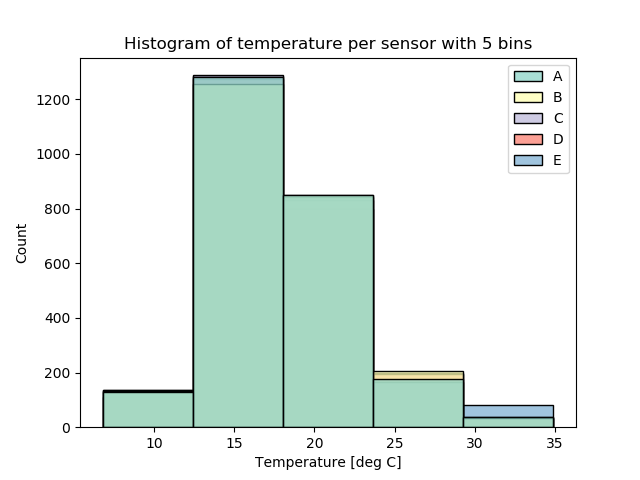
\includegraphics[width=\linewidth]{Histogram of temperature per sensor with 5 bins.png}
		\caption{Histogram of temperature (\degree C) per sensor with 5 bins.}
	\end{subfigure}
	\begin{subfigure}[b]{0.4\linewidth}
		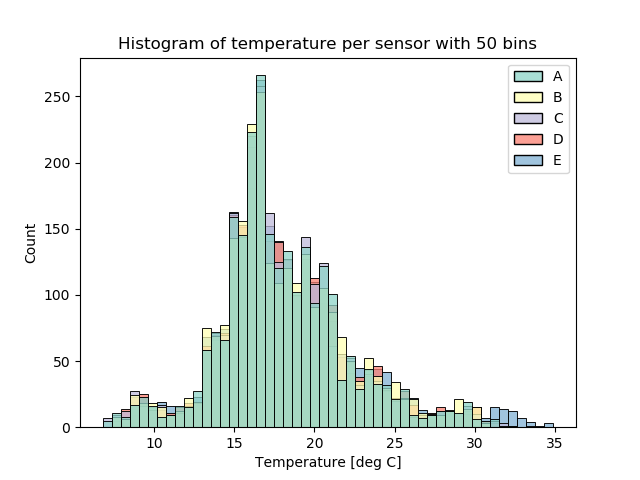
\includegraphics[width=\linewidth]{Histogram of temperature per sensor with 50 bins.png}
		\caption{Histogram of temperature (\degree C) per sensor with 50 bins.}
	\end{subfigure}
	\caption{Histograms of the temperature measured by all 5 sensors in \degree C, with 5 and 50 bins.}
	\label{fig:hist5and50}
\end{figure}


\item {\it Create 1 plot where frequency poligons for the 5 sensors Temperature values overlap in different colors with a legend.}

 \begin{figure}[H] 
    \centering
    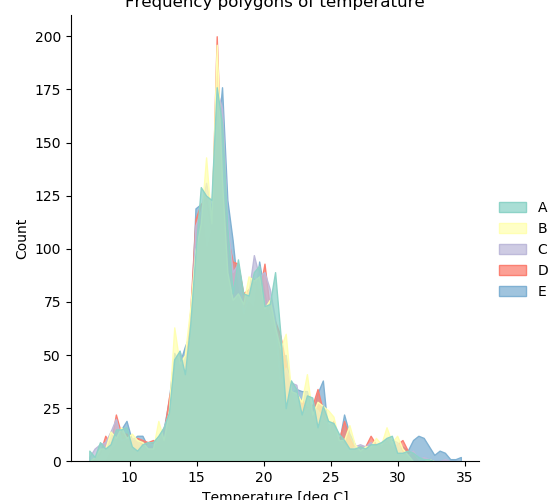
\includegraphics[scale=0.6]{polygon hist temperature.png} 
    \caption{Frequency polygon with 27 bins of the temperature (\degree C) measured by all 5 sensors.} % Creates caption underneath graph
    \label{fig:freqpoly}
  \end{figure}



\item {\it Generate 3 plots that include the 5 sensors boxplot for: Wind Speed, Wind Direction and Temperature.}

 \begin{figure}[H] 
    \centering
    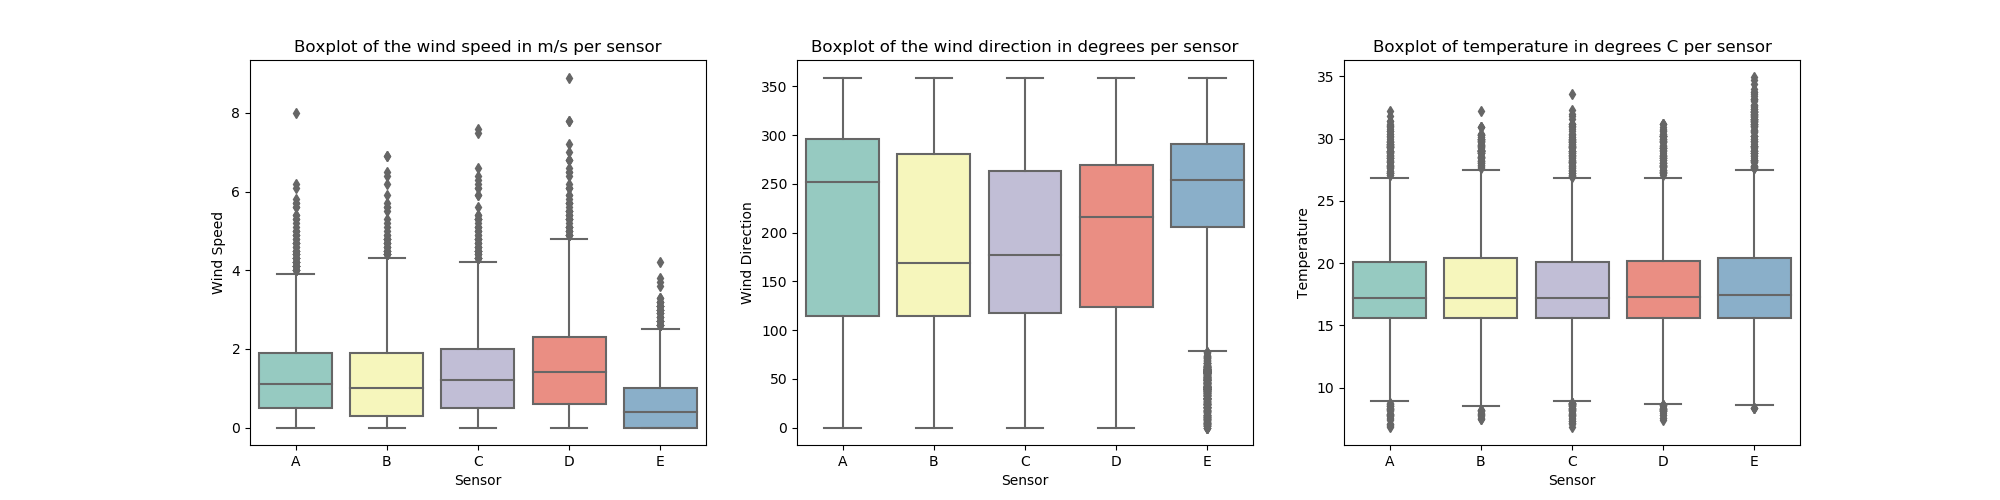
\includegraphics[width=1\textwidth]{Boxplots.png} 
    \caption{Boxplots showing the data distributions for wind speed (m/s), wind direction (deg) and temperature (\degree C).} 
    \label{fig:boxplots}
  \end{figure} 

\item {\it Plot PMF, PDF and CDF for the 5 sensors Temperature values in independent plots (or subplots). Describe the behaviour of the distributions, are they all similar? what about their tails?}

The distribution plotted in figures \ref{fig:PMF}, \ref{fig:PDF}, \ref{fig:CDF} show the distributions of temperature data per sensor. In the first graphs, figure \ref{fig:PMF}, showing the PMF, it can be observed that all 5 sensors are slightly right skewed, and have long tails to the left. In these plots it is also observable that sensor E has the most outliers to the left of the distribution. The PDF plots, figure \ref{fig:PDF}, are very similar to the PMF plots, but outliers in the data have less effect, making it more apparent that the distributions are slightly right skewed with tails to the left. This tail is, similar to the observations in the PMF plot, longest for sensor E. In the bottom plot, figure \ref{fig:CDF}, the CDF plot, the curve resembles an S-curve indicating a relatively normal distribution, however the first part of the curve is relatively flat, indicating only few low temperature values, and the line had a minor kink, indicating a change in frequency of the datapoints. 

 \begin{figure}[H] 
	\centering
	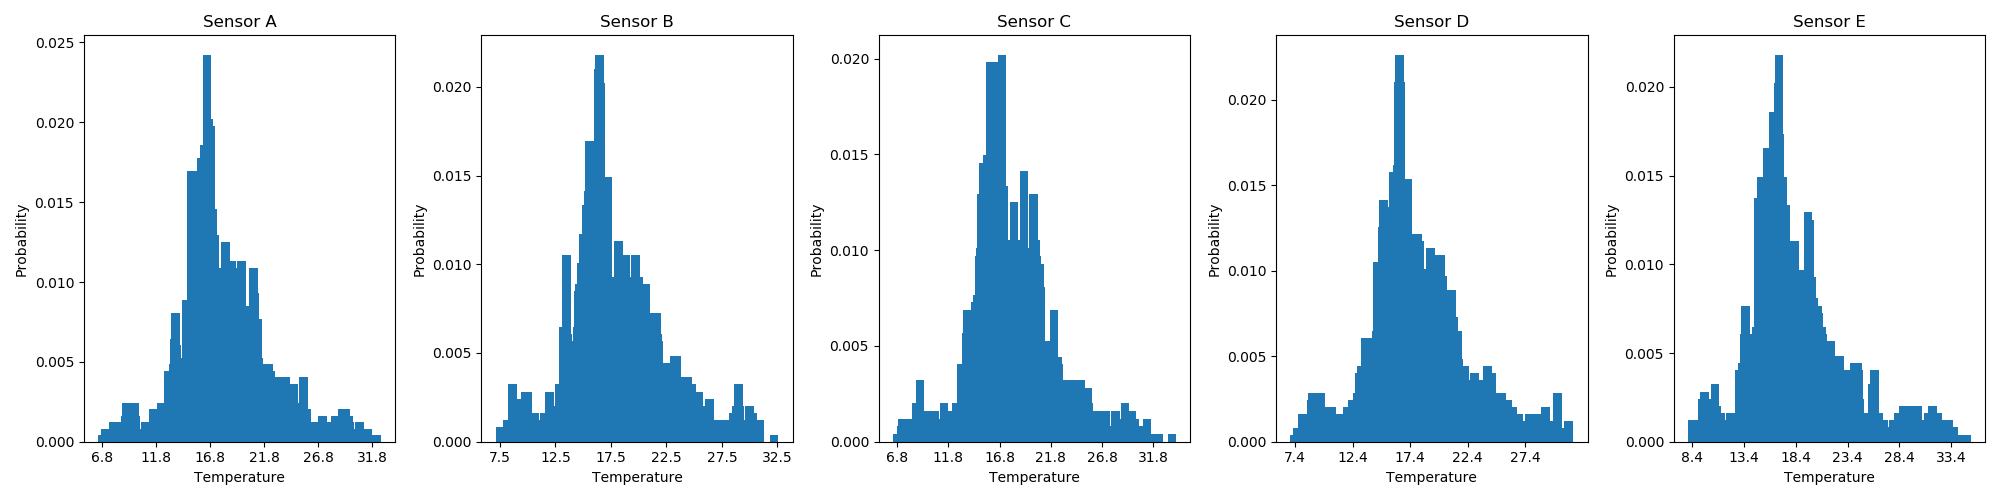
\includegraphics[width=1\textwidth]{PMF of temperature per sensor.png} 
	\caption{Probability Mass Function of the temperature (\degree C) values per sensor.} % Creates caption underneath graph
	\label{fig:PMF}
\end{figure} 

 \begin{figure}[H] 
	\centering
	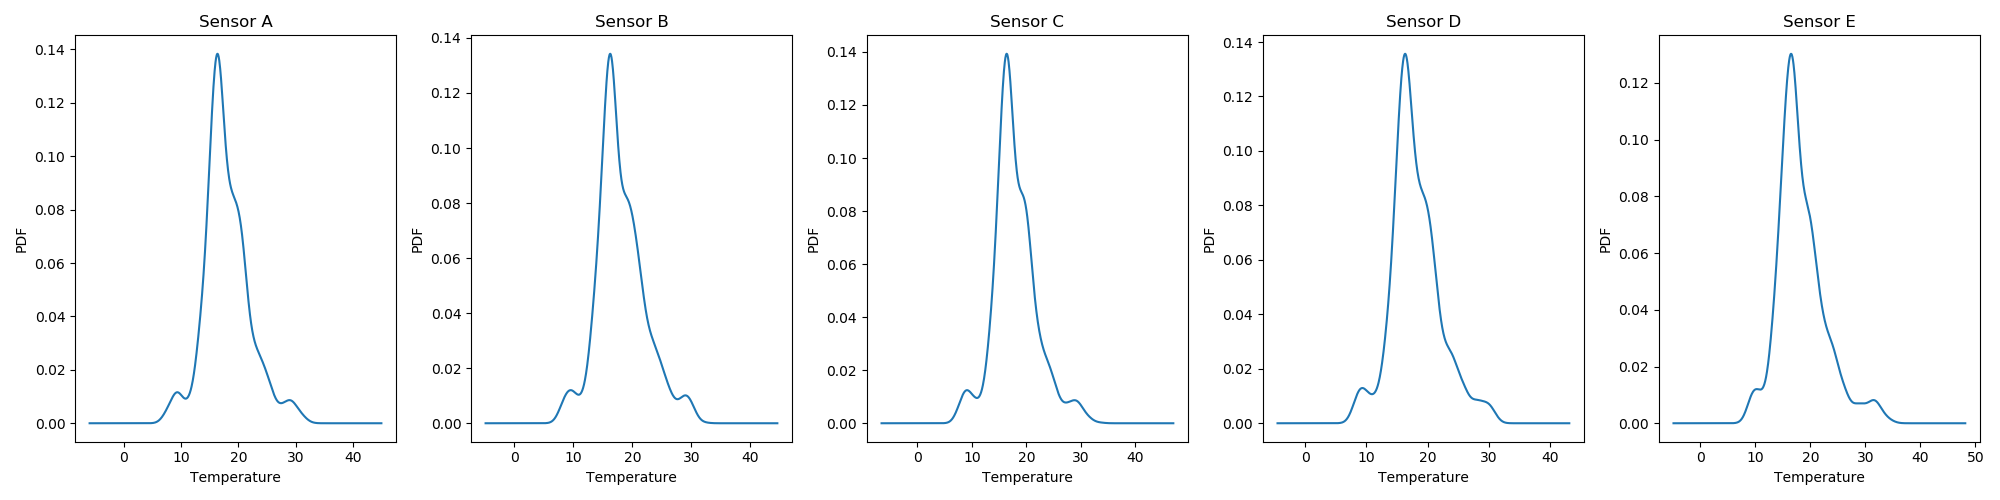
\includegraphics[width=1\textwidth]{PDF of temperature per sensor.png} 
	\caption{Probability Density Function of the temperature values per sensor.} % Creates caption underneath graph
	\label{fig:PDF}
\end{figure} 

 \begin{figure}[H] 
	\centering
	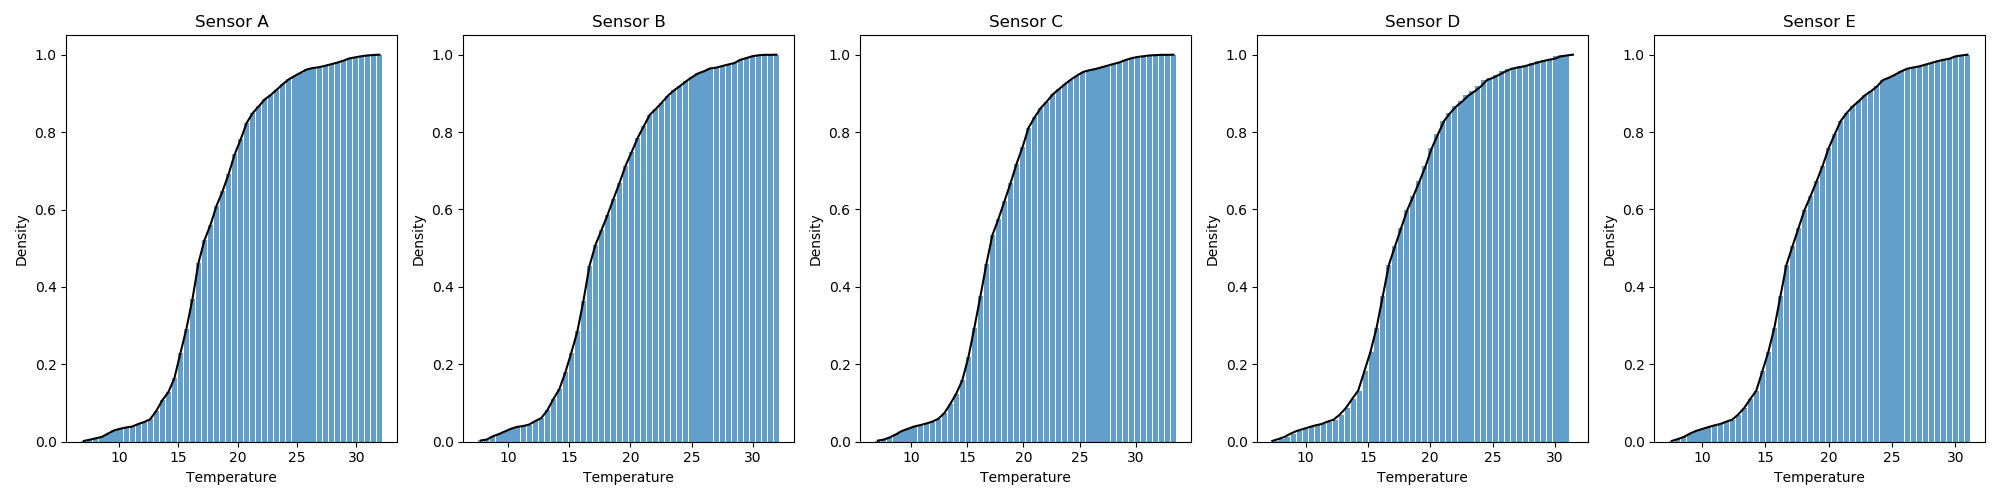
\includegraphics[width=1\textwidth]{CDF of temperature per sensor.png} 
	\caption{Cumulative Density Function of the temperature (\degree C) values per sensor.} % Creates caption underneath graph
	\label{fig:CDF}
\end{figure} 



\item {\it For the Wind Speed values, plot the pdf and the Kernel Density Estimation. Comment the differences}

TEXT 

 \begin{figure}[H] 
	\centering
	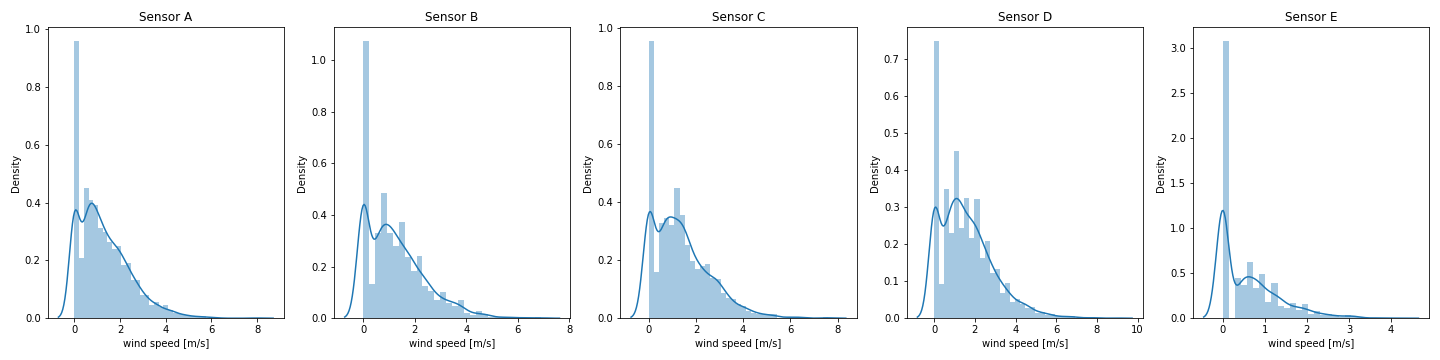
\includegraphics[width=1\textwidth]{KDE and PDF of wind speed per sensor.png} 
	\caption{Probability Density Function (bars) plotted with the kernel density estimation (line) of the wind speed (m/s) measurements per sensor} % Creates caption underneath graph
	\label{fig:PDF+KDE}
\end{figure} 

\item {\it Compute the correlations between all the sensors for the variables: Temperature, Wet Bulb Globe, Crosswind Speed. Perform correlation between sensors with the same variable, not between two different variables; for example, correlate Temperature time series between sensor A and B. Use Pearson’s and Spearmann’s rank coefficients. Make a scatter plot with both coefficients with the 3 variables.}

 \begin{figure}[H] 
    \centering
    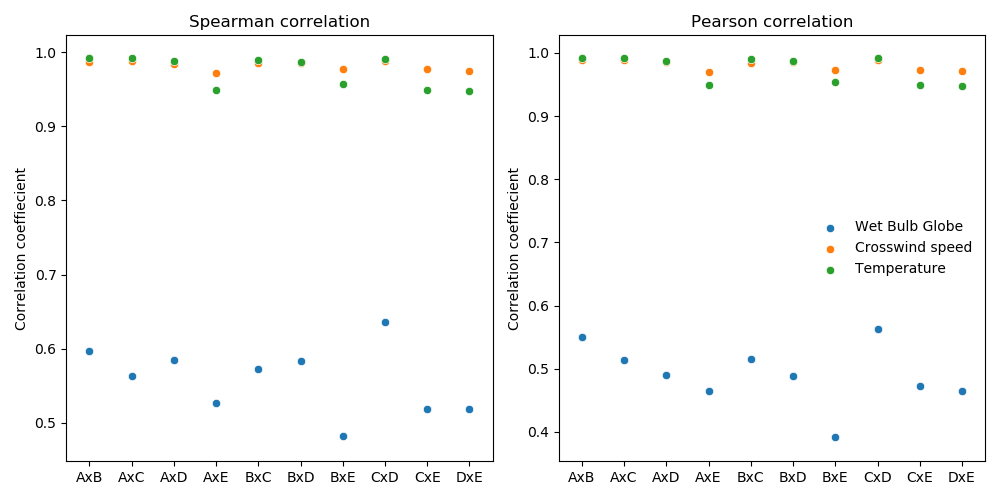
\includegraphics[width=1\textwidth]{Pearson and Spearman correlations.png} 
    \caption{Scatterplot of Spearman and Pearson correlations between sensors dislayed on x-axis.} % Creates caption underneath graph
    \label{fig:corr_scatter}
  \end{figure} 

\item {\it What can you say about the sensors’ correlations?}

When analyzing the correlations it can be observed that the correlations between sensors for the temperature and the wet bulb globe temperature are high, and all sensors correlate strongly with each other on these measurements, as the correlations are above 0.9 and close to 1.0 for both Spearman and Pearson correlations. However, the data from one sensor stands out, sensor E, all correlations between sensor E and another sensor are lower than the correlations between all other sensors. \par

In contrast to the correlations between sensors for temperature and the wet bulb globe temperature, the correlations for crosswind speed are relatively low. Almost all correlations for crosswind speed are below 0.6, except for the spearman correlation between C and D at 0.63, the lowest correlations are, in correspondence with findings for temperature and wet bulb globe temperature with sensor E. 


\item {\it If we told you that that the sensors are located as in figure \ref{fig:sensor_locations}, hypothesize which location would you assign to each sensor and reason your hypothesis using the correlations.}


 \begin{figure}[H] 
	\centering
	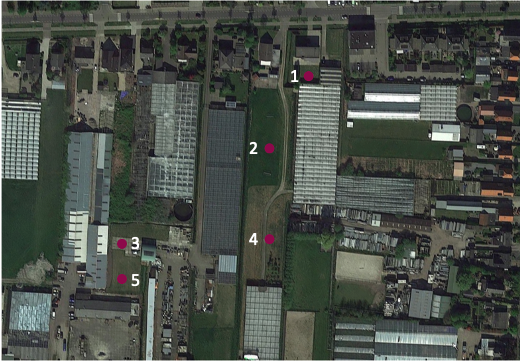
\includegraphics[width=1\textwidth]{Sensor_locations.png} 
	\caption{Numbered locations of sensors on areal photo of Rijsenhout.} 
	\label{fig:sensor_locations}
\end{figure}

where will the sensors be located

\item {\it Plot the CDF for all the sensors and for variables Temperature and Wind Speed, then compute the 95\% confidence intervals for variables Temperature and Wind Speed for all the sensors and save them in a table (txt or csv form).}

\begin{figure}[H] 
	\centering
	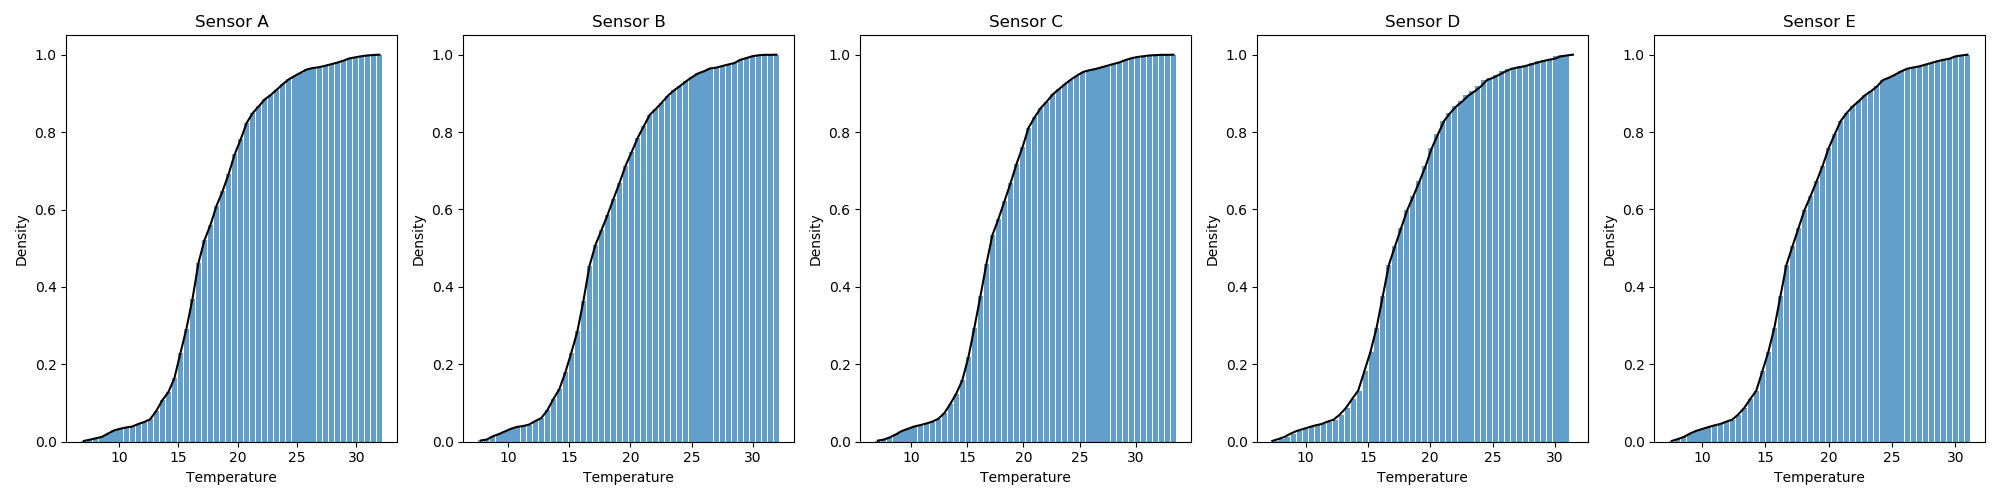
\includegraphics[width=1\textwidth]{CDF of temperature per sensor.png} 
	\caption{Cumulative Density Function of the temperature in \degree C per sensor.} % Creates caption underneath graph
	\label{fig:CDF_T}
\end{figure}  

\begin{figure}[H] 
	\centering
	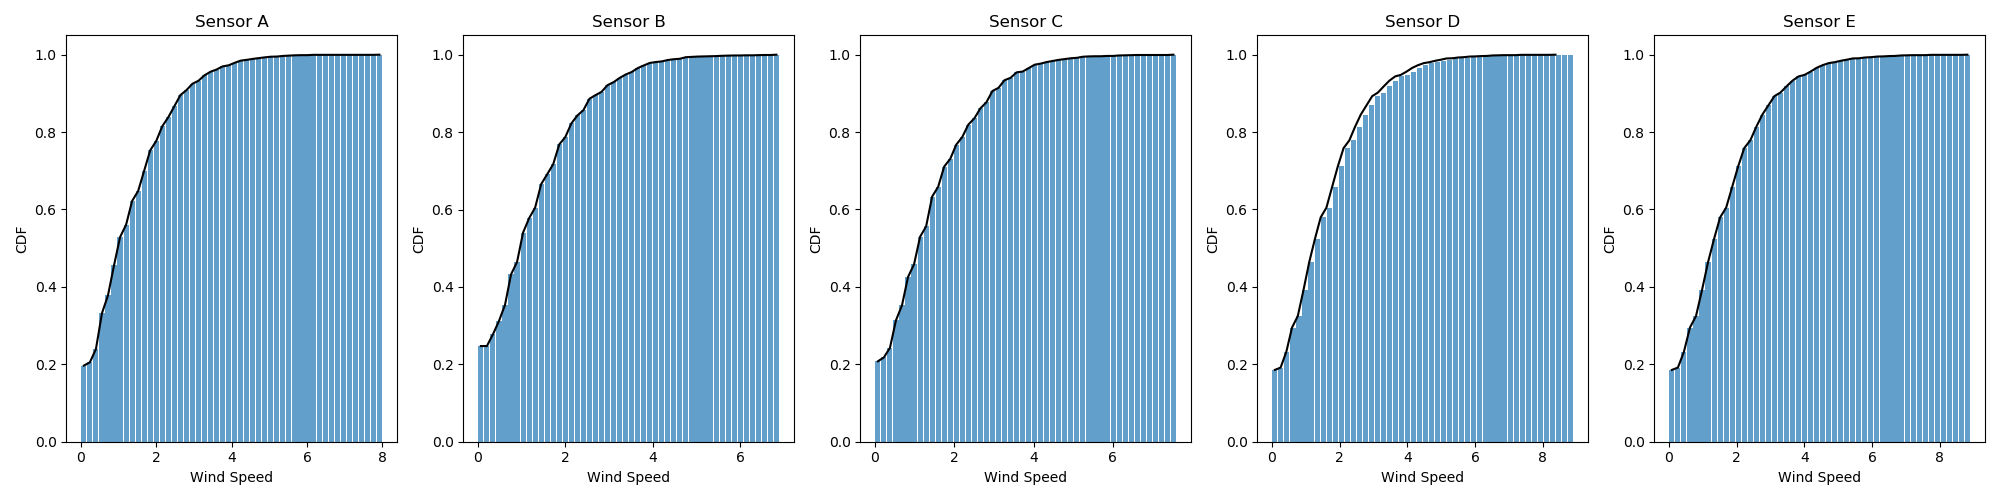
\includegraphics[width=1\textwidth]{CDF of wind speed per sensor.png} 
	\caption{Cumulative Density Function of the wind speed in m/s per sensor.} % Creates caption underneath graph
	\label{fig:CDF_W}
\end{figure} 

The confidence intervals are calculated with the stats.t.interval function from Scipy. This function assumes the data has a student's t distribution, however as seen in question 6, the distribution for the wind speed is right skewed. This led to incorrect negative values for the lower limit of the confidence intervals for the wind speed each sensor, therefore the CDF graphs were used to determine the lower limit at a 95\% confidence level. The plots in \ref{fig:CDF_W} show that about 20\% of the values are 0, hence the value at 2.5\% is 0, therefore this value is used as a lower limit in the confidence interval. The distributions for the temperature values are close to a student's t distribution, and only mildly skewed, hence the values for the confidence interval calculated via te stats.t.interval function do not need to be adjusted. 

\begin{table}[H]
	\centering
	\caption{Confidence intervals for temperature  with 95\% confidence level.}
	\begin{tabular}{llll}
		\multicolumn{1}{c}{\textbf{Sensor}}  & \multicolumn{1}{c}{\textit{Lower limit}} & \textit{Upper limit} \\ \hline
		 A      & 10.160 & 25.778  \\
		B      & 10.071 & 26.060 \\
		C      & 10.045 & 25.781 \\
		D      & 10.128 & 25.864 \\
		E      & 9.799  & 26.909 
	\end{tabular}
\label{CI_T}
\end{table}

\begin{table}[H]
	\centering
	\caption{Confidence intervals for wind speed with a 95\% confidence level.}
	\begin{tabular}{llll}
		\multicolumn{1}{c}{\textbf{Sensor}}  & \multicolumn{1}{c}{\textit{Lower limit}} & \textit{Upper limit} \\ \hline
		 A      & 0              & 3.483 \\
		 B      & 0              & 3.479   \\
		 C      & 0              & 3.717  \\
		 D      & 0              & 4.168  \\
		 E      & 0              & 1.998
	\end{tabular}
\label{CI_WS}
\end{table}

\item {\it Test the hypothesis: the time series for Temperature and Wind Speed are the same for sensors:}

\begin{table}[H]
	\centering
	\caption{t-statistic and p-values of the tested sensor pairs for temperature}
	\begin{tabular}{lll}
			\multicolumn{1}{c}{\textbf{Sensor pair}}  & \multicolumn{1}{c}{\textit{t-statistic}} & \textit{p-value} \\ \hline
		E-D & 16.750  & \num{9.731e-60}  \\
		D-C & 6.875   & \num{7.843e-12}  \\
		C-B & -10.581 & \num{1.274e-25} \\
		B-A & 7.598   & \num{4.24e-14}
	\end{tabular}
\label{hypo_test_T}
\end{table}

\begin{table}[H]
	\centering
	\caption{t-statistic and p-values of the tested sensor pairs for wind speed}
	\begin{tabular}{lll}
		\multicolumn{1}{c}{\textbf{Sensor pair}}  & \multicolumn{1}{c}{\textit{t-statistic}} & \textit{p-value} \\ \hline
	E-D & -44.709 & \num{1.839e-320}             \\
	D-C & 9.537  & \num{3.374e-21}  \\
	C-B & 6.069    & \num{1.486e-09} \\
	B-A & -2.485 & 0.013
	\end{tabular}
	\label{hypo_test_W}
\end{table}



\item {\it What could you conclude from the p-values?}

The hypothesis test are done with the stats.ttest\_rel function from Scipy, as the samples are measures at the same location and are therefore not truly independent. The p-values for all hypothesis tests for the temperature and wind speed are below 0.025, and therefore should the null hypothesis that the tested sensors have identical means be rejected.

\item {\it Bonus:\\ Your “employer” wants to estimate the day of maximum and minimum potential energy consumption due to air conditioning usage. To hypothesize regarding those days, you are asked to identify the hottest and coolest day of the measurement time series provided. How would you do that? Reason and program the python routine that would allow you to identify those days}

Code van bonus question en info 



\begin{verbatim}
	If you have code put it here
\end{verbatim}

% You just have to exchange the x for the right value.

\end{enumerate}

% You might use the part below if you have extensive code to share

% \clearpage
% \section*{Python Code}

% \begin{verbatim}
% Put any big code you have here.

% \end{verbatim}

\bibliographystyle{plain}
\bibliography{bibliography}


\end{document}
